\chapter{Regelungstechnische Ansätze}\label{cha:GrundlagenReg}
Nachdem die Modellimplementierung vollständig beschrieben wurde, sollen nun einige regelungstechnischen Grundlagen zur Verkopplungsregelung erläutert werden. Für den Reglerentwurf wird die institutseigene Toolbox \texttt{gammasyn} verwendet. Diese soll einen robusten Verkopplungsentwurf ermöglichen. Hierfür wird die auf dem Multi-Model-Ansatz basierende Polbereichsplatzierung mit dem Verkopplungsentwurf über Invarianzbetrachtungen kombiniert. Für eine genauere Beschreibung der Toolbox sei auf die Dokumentation verwiesen\cite{Vogt, gammaDoku}.
Im folgenden Kapitel wird zunächst auf das Vorgehen bei der Polbereichsplatzierung eingegangen, um anschließend die Theorie hinter dem Verkopplungsentwurf mittels invarianten Unterräumen zu skizzieren.

\section{Polbereichsplatzierung}\label{sec:PBV}
In realen System kommt es immer zu Unsicherheiten oder Veränderungen welche das System- und Regelverhalten beeinflussen.
Die Methode der Polbereichsplatzierung, basierend auf dem  Multi-Modell-Ansatz, versucht die lineare Zustandsregelung von Systemen mit schwankenden oder unsicheren Parametern zu ermöglichen.
Die Erklärungen im nachfolgenden Abschnitt basieren auf den Ausführungen in \cite{RobReg} und \cite{Schaub}.

Zunächst wird das System in Abhängigkeit eines Parametervektors $\Theta$ wie folgt definiert
\begin{align}
	\dot{\w{x}} &= \M{A}(\Theta)\w{x} + \M{B}(\Theta)\w{u}\, , \qquad \w{x}(0) = \w{x}_0\\
	\w{y} 		&= \M{C}(\Theta)\w{x}
\end{align}
Das System besitzt die Ordnung $n$. Des Weiteren gilt $\w{u}\in\mathbb{R}^p$ und $\w{y}\in\mathbb{R}^q$. Es sind also $p$ Stellgrößen und $q$ Ausgangsgrößen vorhanden.
Der Parametervektor $\Theta$ beschreibt die veränderlichen Parameter des Systems. Beim Multi-Modell-Ansatz wird nun das System an $\Omega$ Stützstellen um $\Theta_{\rho}$ linearisiert. Somit erhält man eine Menge an $\Omega$ Systemmodellen, welche sich mit $\rho = 1,...,\Omega$ zu 
\begin{align}
	\dot{\wr{x}} &= \Mr{A} \wr{x} + \Mr{B}\w{u}\, , \qquad \wr{x}(0) = \w{x}_{0\rho}\\
	\wr{y} 		 &= \Mr{C}\wr{x}
\end{align}
definieren lassen.\\
Die Lage der Eigenwerte des geschlossenen Regelkreises bestimmen dessen Dynamik, also Dämpfung, Schnelligkeit oder Schwingverhalten. In Abbildung \ref{fig:BedPolgebGrenzen} wird veranschaulicht, wie unterschiedliche Polgebietsgrenzen diese Dynamik beeinflussen. 
\begin{figure}[h]
	\centering
	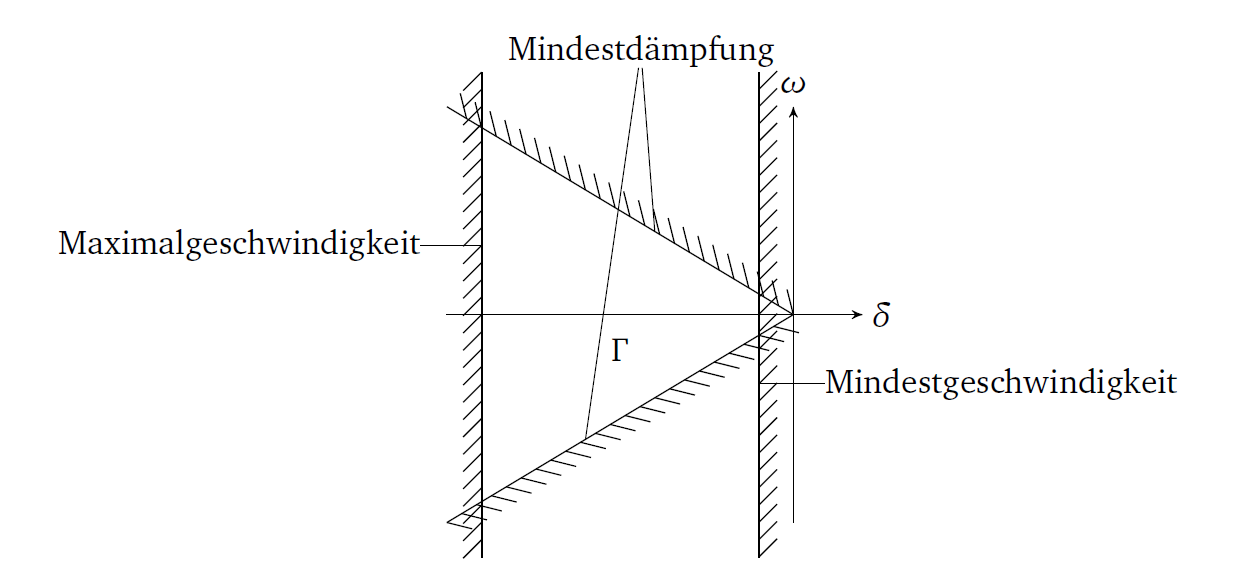
\includegraphics[width=\textwidth]{./Bilder/BedPolgebGrenzen.png}
	\caption{Bedeutung der Polgebietsgrenzen.\cite{RobReg}}
	\label{fig:BedPolgebGrenzen}
\end{figure}
Die Achsen beschreiben mit $\delta$ und $\omega$ den Real- bzw. Imaginärteil eines Poles $\lambda = \delta +\textnormal{j}\omega$.
Ziel ist nun einen Regler $\M{R}$ zu finden, welcher mit einer konstanten Zustandsrückführung alle Eigenwerte der verschiedenen Systeme in den vorher definierten Bereich $\Gamma$ platziert.
Über die Gebietsgrenzen von $\Gamma$ werden Anforderungen an Regel- bzw. Systemdynamiken entsprechend obiger Grafik \ref{fig:BedPolgebGrenzen} vorgegeben.
%, wie z.B. Schnelligkeit oder Schwingverhalten, vorgegeben werden.
Dabei kann es auch sinnvoll sein, unterschiedliche Polgebiete für die einzelnen Modelle zu definieren. Genauere Erklärungen zur mathematischen Beschreibung der Polgebietsgrenzen findet sich in entsprechender Literatur \cite{RobReg}.

Für das Verfahren ist es also nötig zu bewerten, wie gut die Fähigkeit eines bestimmten Reglers $\M{R}$ ist, die Eigenwerte des geregelten Systems im definierten Gebiet $\Gamma$ zu platzieren.
Hierfür soll eine Gütefunktion $J$ definiert werden. 
%Diese soll in Abhängigkeit von $\M{R}$ bewerten wie gut die Fähigkeit eines bestimmten Reglers ist die Eigenwerte des geregelten System im definierten Gebiet $\Gamma$ zu platzieren.
Seien die Eigenwerte des geregelten Systems gegeben durch 
$\lambda_{\rho i}(\M{R}) = \delta_{\rho i} (\M{R}) + \textnormal{j} \omega_{\rho i}(\M{R}) $ 
mit $\rho = 1,...,\Omega$ und $i = 1, ..., n$.
So soll gelten $\lambda_{\rho i}(\M{R}) \in \Gamma$. Liegen die Eigenwerte außerhalb des Bereichs, so soll $J(\M{R})$ große Werte annehmen.
Daraus lässt sich folgende Funktion 
\begin{equation}
	f\left(\delta_{\rho i}(\M{R}) ,\omega_{\rho i}(\M{R})\right) 
	\begin{cases}
		> 0 , \textnormal{wenn } \lambda_{\rho i}(\M{R}) \textnormal{ außerhalb von } \Gamma \textnormal{ liegt} \\
		= 0 , \textnormal{wenn } \lambda_{\rho i}(\M{R}) \textnormal{ auf dem Rand von } \Gamma \textnormal{ liegt} \\
		< 0 , \textnormal{wenn } \lambda_{\rho i}(\M{R}) \textnormal{ innerhalb von } \Gamma \textnormal{ liegt} \\
	\end{cases}
\end{equation}
ableiten.
Eine mögliche Gütefunktion ergibt sich dann zu 
\begin{equation}\label{eq:GueteMExp}
	J(\M{R}) = \sum_{\rho = 1}^{\Omega} \sum_{i=1}^{n} \mathrm{e}^{p_\rho f\left(\delta_{\rho i}(\M{R}) ,\omega_{\rho i}(\M{R})\right)}\,,
\end{equation}
wobei $p_\rho$ ein Gewichtungsfaktor darstellt.
Zur Lösung des Optimierungsproblems muss ein Regler $\M{R}^*$ gefunden werden, welcher die Gütefunktion $J(\M{R})$ minimiert.
\begin{equation}
	\M{R}^* = \textnormal{arg} \min_{\M{R}} J(\M{R})
\end{equation}
Für dieses nichtkonvexe Optimierungsproblem, ist ein numerisches Lösungsverfahren nötig.
Hier werden in der Regel Gradientenverfahren verwendet. Diese nutzen den Gradienten $\frac{\partial J(\M{R})}{\partial \M{R}}$ von $J$, um schrittweise das Minimum der Gütefunktion zu berechnen.\\
Der Gradient ergibt sich elementweise zu
\begin{equation}
	\frac{\partial J(\M{R})}{\partial r_{jh}} = \sum_{\rho = 1}^{\Omega} \sum_{i=1}^{n}
	p_\rho \mathrm{e}^{p_\rho f\left(\delta_{\rho i} ,\omega_{\rho i}\right)}
	\left(
	\frac{\partial f(\delta_{\rho i} ,\omega_{\rho i})}{\partial \delta_{\rho i}}
	\frac{\partial \delta_{\rho i} }{\partial r_{jh}} +
	\frac{\partial f(\delta_{\rho i} ,\omega_{\rho i})}{\partial \omega_{\rho i}}
	\frac{\partial \omega_{\rho i}}{\partial r_{jh}}
	\right)
\end{equation}
Hierbei gilt $j = 1,..,p$ und $h = 1,...,n$. Die Ableitungen $\frac{\partial f(\delta_{\rho i} ,\omega_{\rho i})}{\partial \delta_{\rho i}}$ sowie $	\frac{\partial f(\delta_{\rho i} ,\omega_{\rho i})}{\partial \omega_{\rho i}}$ ergeben sich aus den Grenzkurvenfunktionen des definierten Polgebiets $\Gamma$.
Zur Bestimmung von $\frac{\partial \delta_{\rho i} }{\partial r_{jh}} $ und $\frac{\partial \omega_{\rho i}}{\partial r_{jh}}$ nutzt man folgenden Zusammenhang
\begin{equation}
	\frac{\partial \lambda_{\rho i} }{\partial r_{jh}} = 	
	\frac{\partial \delta_{\rho i} }{\partial r_{jh}} +
	\textnormal{j}\frac{\partial \omega_{\rho i}}{\partial r_{jh}}
	\eqp
\end{equation}
Die Ableitungen ergeben sich dann zu 
\begin{equation}
		\frac{\partial \delta_{\rho i} }{\partial r_{jh}} = \Re\left\{ \frac{\partial \lambda_{\rho i} }{\partial r_{jh}}  \right\}
		\qquad \textnormal{und} \qquad
		\frac{\partial \omega_{\rho i}}{\partial r_{jh}} = \Im\left\{ \frac{\partial \lambda_{\rho i} }{\partial r_{jh}} \right\}
\end{equation}
Es gilt also $\frac{\partial \lambda_{\rho i} }{\partial r_{jh}}$ zu berechnen. Dies geschieht durch die beidseitige Ableitung des Rechtseigenwertproblems 
\begin{equation}
	\left( \M{A} - \M{B}\M{R} \right)\wt{v}{R i} = \lambda_{R i}\wt{v}{R i}
\end{equation}
nach einem Regelparameter $r_{jh}$. Bei vollständiger Zustandsrückführung ergibt sich die Ableitung dann zu
\begin{equation}\label{eq:AblLambdaR}
	\frac{\partial \lambda_{\rho i} }{\partial r_{jh}} = 
	- \frac{\w{w}^{\textnormal{T}}_{R i} \M{B} \wt{e}{j} \w{e}^{\textnormal{T}}_k \wt{v}{R i} }
		   {\w{w}^{\textnormal{T}}_{R i}  \wt{v}{R i}}
	\eqp
\end{equation}
Hier handelt es sich bei $\wt{w}{R i}$ um den $i-$ten Linkseigenvektor und bei $ \wt{v}{R i}$ um den entsprechenden Rechtseigenvektor. Die Vektoren $\wt{e}{j}$ und $\wt{e}{k}$ bezeichnen Einheitsvektoren in die $j-$te bzw. $k-$te Koordinatenrichtung.

Mit den Gleichungen (\ref{eq:GueteMExp}) und (\ref{eq:AblLambdaR}) kann nun ein optimaler Regler entworfen werden. Insgesamt können durch diese Methode alle $p\cdot n$ Koeffizienten in $\M{R}$ berechnet werden. Es ist jedoch auch möglich das Verfahren in Kombination mit strukturbeschränkten Reglern zu verwenden. Hierfür muss lediglich die Anzahl an Optimierungsvariablen  reduziert werden. Damit verändert man nicht mehr alle Reglerkoeffizienten in der Optimierung und es ist möglich, bestimmte Parameter fest oder von anderen abhängig zu wählen.

Nach dem Reglerentwurf ist eine Überprüfung der exakten Lage der Pole nötig. Dies soll sicherzustellen, dass alle Pole wie in Abbildung \ref{fig:PolgebKorrekt} dargestellt innerhalb des gewünschten Gebiets $\Gamma$ liegen. Tritt der in Abbildung \ref{fig:PolgebFalsch} beschriebene Fall auf, so muss der Reglerentwurf optimiert werden bis man zufriedenstellende Ergebnisse erzielt. In der Regel geschieht dies durch Änderung der Startwerte oder Gewichtungsfaktoren oder Polbereichsanpassungen.

\begin{figure}[h]
	\centering
	\begin{subfigure}[b]{0.35\textwidth}
		\centering
		\includegraphics[width=\textwidth]{./Bilder/PolgebKorrekt.png}
		\caption{Alle Pole der geregelten Strecke liegen innerhalb von $\Gamma$}
		\label{fig:PolgebKorrekt}
	\end{subfigure}
	\hspace{0.1\textwidth}
	\begin{subfigure}[b]{0.35\textwidth}
		\centering
		\includegraphics[width=0.85\textwidth]{./Bilder/PolgebFalsch.png}
		\caption{Einige Pole der geregelten Strecke liegen außerhalb von $\Gamma$}
		\label{fig:PolgebFalsch}
	\end{subfigure}
	\caption{Polgebiete mit Regelungseigenwerten \cite{Schaub}.}
	\label{fig:PolGeb}
\end{figure}
Nachdem das Konzept der Polbereichsplatzierung beschrieben wurde, soll im nächsten Abschnitt das Vorgehen bei der robusten Verkopplungsregelung auf Basis von Invarianzbetrachtungen erklärt werden.\\


\section{Verkopplungsregelung}\label{sec:Verkopplung}

Die Erläuterungen in diesem Abschnitt sind an den Erklärungen in der Arbeit "Robuster Verkopplungsreglerentwurf mittels Polbereichsvorgabe" von Schaub \cite{Schaub} angelehnt. Dabei wird hier bewusst auf die Darstellung von Beweisen verzichtet, um die Erklärungen möglichst knapp und übersichtlich zu gestalten.

Für den Reglerentwurf muss zunächst das robuste Verkopplungsproblem definiert werden.
Hierfür lassen sich die aus dem Multi-Modell-Ansatz resultierenden dynamischen Systeme wie folgt umformulieren
\begin{align}
	\underline{\dot{x}}_{\rho}  &= \textbf{A}_\rho \underline{x}_{\rho} + \textbf{B}_\rho \underline{u}_{\rho}, \qquad \underline{x}_{\rho}(0) = \underline{x}_{0\rho} \\
	\underline{y}_{\rho} &= \textbf{C}_\rho\underline{x}_{\rho} = \begin{bmatrix}\textbf{C}_{1\rho} \\ \textbf{C}_{2\rho} \end{bmatrix} \underline{x}_{\rho}
\end{align}

Genau wie beim Multi-Model-Ansatz gilt dabei $\wt{x}{\rho}\in \mathbb{R}^{n},\, \w{u}\in \mathbb{R}^{p},\, \wt{y}{\rho}\in \mathbb{R}^{q}$ und $\rho = 1, ..., \Omega$.\\
Zudem sind in den Matrizen $\Mt{C}{2\rho}$ die Parameter von jeweils $l$ Verkopplungsbedingungen
\begin{align}\label{eq:Koppl}
	\wt{y}{2\rho} = \Mt{C}{2\rho} \wt{x}{\rho} \stackrel{!}{=} \M{0}
\end{align}
definiert.
Ziel ist es nun eine konstante Zustandsrückführung mit Vorfilter
\begin{equation}\label{eq:uINV}
	\w{u} = -\M{R}\wt{x}{\rho} + \M{F}\w{w} = -\M{R}\wt{x}{\rho} + \begin{bmatrix}\Mt{F}{1} & \Mt{F}{2} \end{bmatrix} \w{w}
\end{equation}
zu finden, welche die Verkopplungsbedingungen erfüllt und alle Eigenwerte im gewünschten Polbereich platziert.
Dabei ist es nicht möglich die klassische Verkopplung mittels vollständiger Modaler Synthese zu nutzen. Dies liegt daran, dass hier der Verkopplungsentwurf und die Eigenwertvorgabe nicht getrennt sind \cite{Schaub}. Somit wäre die Polbereichsplatzierung nicht durchführbar. 
Darum wird für die robuste Verkopplung das Verfahren mittels Invarianzbetrachtung genutzt.
Dafür ist $\M{R}$ und $\M{F}$ in Gleichung (\ref{eq:uINV}) so zu wählen, dass für jedes zu betrachtende System $(\Mt{A}{\rho}-\Mt{B}{\rho}\M{R})$, paarweise verschiedene Eigenwerte erzeugt werden, welche $m_\rho$ Rechtseigenvektoren im Kern von $\Mt{C}{2\rho}$ besitzen. Die restlichen $n-m_\rho$ Eigenwerte sollen über das Vorfilter $\M{F}_1$ von $\w{w}$ aus nicht steuerbar sein. Dies entspricht der eingangsseitigen Verkopplungsbedingung.
Die Variable $m_\rho \in \mathbb{N}$ bezeichnet hier die Dimension des größten geregelten invarianten Unterraums $\mathcal{Q}_\rho$ innerhalb des Kerns von $\Mt{C}{2\rho}$.

Vereinfacht gesagt, muss die Regelung dafür sorgen, dass der Zustand $\w{x}$ den Unterraum $\mathcal{C} = \textnormal{ker}(\Mt{C}{2\rho})$ nicht mehr verlässt sobald er ihn betritt.
Denn die Verkopplungsbedingung (vgl. Gl. (\ref{eq:Koppl})) ist genau dann erfüllt wenn $\w{x} \in \mathcal{C} $.\\
Dieser Zusammenhang soll kurz an einem Beispiel veranschaulicht werden.
Gegeben sei ein dynamische System 3ter Ordnung mit dem Zustandsvektor $x = \begin{bmatrix}
\wt{x}{1} &\wt{x}{2} &\wt{x}{3} \end{bmatrix}^{\textnormal{T}}$.
Zudem gelte die Verkopplungsbedingung $x1 \stackrel{!}{=} x2$. Diese lässt sich analog zu Gleichung (\ref{eq:Koppl}) durch 
\begin{equation}\label{eq:KopplBsp}
	\wt{y}{2} = \begin{bmatrix}
		1 &-1 &0
	\end{bmatrix} \w{x} = \Mt{C}{2}\w{x} \stackrel{!}{=} 0 
\end{equation}\\
ausdrücken.\\
In Abbildung \ref{fig:UnterRTraj} ist der Rechtskern von $\Mt{C}{2}$ als graue Ebene gekennzeichnet. Außerdem eine zulässige Trajektorie $\w{x}(t)$, welche die Verkopplungsbedingung (\ref{eq:KopplBsp}) erfüllt. Die Grafik verdeutlicht, dass die Erfüllung der Verkopplungsbedingung gegeben ist, sobald $\w{x}(t)$ in die graue Ebene eintritt und diese nicht mehr verlässt. 

\begin{figure}[h]
	\centering
	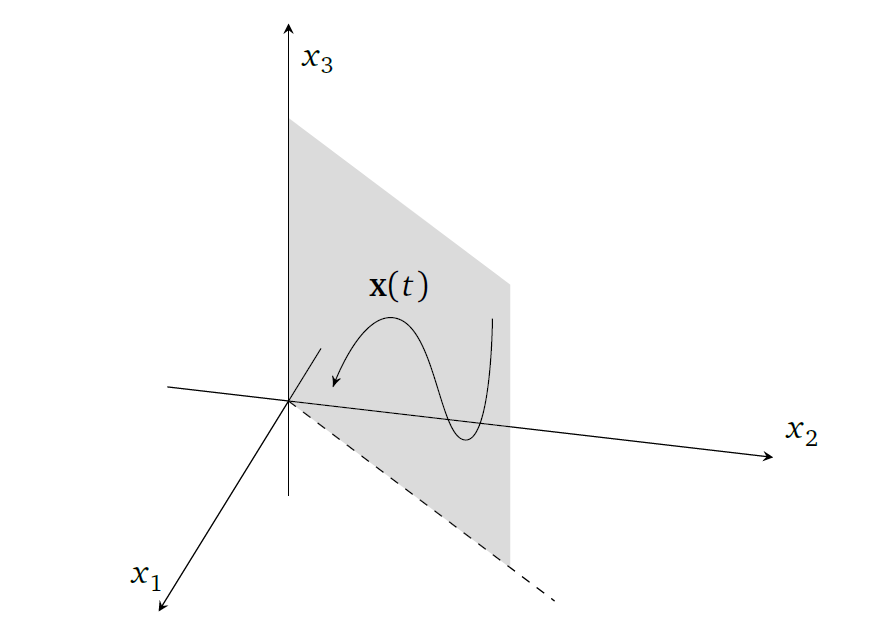
\includegraphics[width=\textwidth]{./Bilder/UnterraumTraj.png}
	\caption{Unterraum von $\Mt{C}{2}$ mit zulässiger Trajektorie $\w{x}(t)$ \cite{Schaub}.}
	\label{fig:UnterRTraj}
\end{figure}
Demnach lässt sich das Verkopplungsproblem als Forderung nach geregelter Invarianz interpretieren, wobei der Zusammenhang
\begin{equation}
	(\M{A}-\M{B}\M{R})\mathcal{C} \subseteq \mathcal{C}  
\end{equation}
zwar wünschenswert, aber in der Regel nicht erreichbar ist. Dies liegt daran, dass $\mathcal{C}$ nicht zwingend geregelt invariant ist. Daher muss zunächst der größte geregelte invariante Unterraum $\mathcal{Q} \in \mathcal{C}$ bestimmt werden. Dessen Dimension $m$ beschreibt die Anzahl an Eigenvektoren, welche die ausgangsseitige Verkopplungsbedingung erfüllen. 
Der Unterraum $\mathcal{Q}$ definiert dabei über 
\begin{equation}
	(\M{A} - \M{B}\M{R}) \mathcal{Q} \subseteq \mathcal{Q}
\end{equation}
die Freiheitsgrade des Reglers $\M{R}$, welche benötigt werden, um das Verkopplungsproblem zu lösen. Für eine einfachere Bestimmung der Freiheitsgrade wird zunächst der Zustandsraum durch
\begin{equation}
	\w{x} = \M{V}\w{\tilde{x}}
\end{equation}
transformiert.
Dabei sollen die ersten $m$ Koordinatenachsen an der Basis von $\mathcal{Q}$ ausgerichtet werden.
Dies geschieht mit Hilfe der Transformationsmatrix 
\begin{equation}
\M{V} =\begin{bmatrix} \M{Q}	&\M{Q}_{\bot} \end{bmatrix}
\end{equation}
wobei $\M{Q}_{\bot}$ die Dimension $(n \times (n-m))$ besitzt. Die einfachste Möglichkeit einer solchen regulären Transformation ist
\begin{equation}
		\M{Q}^{\textnormal{T}} \M{Q}_{\bot} = \M{0} \eqp
\end{equation}
Ist der Zustandsraum ausgerichtet, so hat der transformiert Zustandsvektor $\w{\tilde{x}}$ folgende Form
\begin{equation}
	\w{\tilde{x}} = \begin{bmatrix}
		\tilde{x}_1 &\dots &\tilde{x}_m &0 &\dots &0
	\end{bmatrix}^{\textnormal{T}}
\end{equation} 
%EVTL. ABB von Ebene mit gedrehten Achsen\\
und die Systemmatrix ergibt sich zu
\begin{equation}
	\Mtilt{A}{r}(\M{R}) = \M{V}^{-1}(\M{A} - \M{B}\M{R})\M{V} = \begin{bmatrix}
		\Mtilt{A}{11}(\M{R})	&\Mtilt{A}{12}(\M{R})	\\
		\Mtilt{A}{21}(\M{R})	&\Mtilt{A}{22}(\M{R})
	\end{bmatrix} \eqp
\end{equation}
Soll $\mathcal{Q}$ invariant unter $\Mtilt{A}{r}(\M{R})$ sein, dann muss
\begin{equation}\label{eq:BedGl}
	\Mtilt{A}{21}(\M{R}) = \M{0} 
\end{equation}
gelten.
Da $\Mtilt{A}{21}(\M{R}) \in \mathbb{R}^{(n-m)\times m} $ gilt, lassen sich aus dieser Bedingung $(n-m)\cdot m$ lineare Gleichungen für die Reglerparameter ableiten.


Zur Lösung dieses Gleichungssystems soll es in eine Matrixform gebracht werden.
Dafür bringt man die Regelparameter aus
\begin{equation}
	\M{R} = \begin{bmatrix}
		r_{11} &\dots &r_{1n} \\
		\vdots &\ddots &\vdots \\
		r_{p1} &\dots &r_{pn}
	\end{bmatrix}
\end{equation}
in folgende Form
\begin{equation}
	\w{r} = \textnormal{vec}(\M{R}) = \begin{bmatrix} r_{11} &\dots &r_{p1} &\dots &r_{1n} &\dots &r_{pn} 	\end{bmatrix}^{\textnormal{T}} \eqp
\end{equation}
Anschließend werden die durch (\ref{eq:BedGl}) definierten Bedingungsgleichungen in der Matrixform
\begin{equation}\label{eq:GlSysM}
	\M{X}\w{r} = \w{z}
\end{equation}
zusammengefasst.

Bei einer robusten Verkopplung muss dieses Verfahren dann für alle $\Omega$ Modelle durchgeführt werden. Dabei beschreibt 
\begin{equation}
	\M{X}_\rho\w{r} = \w{z}_\rho \eqp
\end{equation}
das Gleichungssystem des $\rho$-ten Modells.
Die Gesamtheit der Gleichungssysteme lässt sich dann zu 
\begin{equation}\label{eq:GesGlSysM}
	\M{X}_R \w{r} = \w{z}_R \qquad \textnormal{ mit } \M{X}_R = 
	\begin{bmatrix}	\M{X}_1\\ \vdots\\ \M{X}_\Omega	\end{bmatrix}
	\qquad \textnormal{und }  \w{z}_R
	\begin{bmatrix}	\w{z}_1\\ \vdots\\ \w{z}_\Omega	\end{bmatrix}
\end{equation}
definieren.
Existiert keine Lösung für das Gesamtgleichungssystem, dann ist es nicht möglich mit einer konstanten Zustandsrückführung die Verkopplungsbedingungen für alle Modelle gleichzeitig zu erfüllen.
Existiert hingegen eine Lösung, so ergeben sich Strukturbeschränkungen für den Regler $\M{R}$. 
Der Lösungsraum von $\w{r}$ definiert hier die Struktur über affine Abhängigkeiten der Reglerparameter untereinander.

Um die robuste Verkopplung zu vervollständigen, gilt es nun das Vorgehen zur Bestimmung der Strukturbeschränkungen des Vorfilters genauer zu betrachten.
Hierfür muss, wie bereits erwähnt, $\M{F}_1$ so gestaltet werden, dass die restlichen $n-m_\rho$ Eigenwerte von \w{w} aus nicht steuerbar sind.

Dies ergibt die eingangsseitige Verkopplungsbedingung
\begin{equation}\label{eq:EingKoppl}
	\M{W}_{R2}\M{B}\M{F}_1 = \M{0} \qquad \textnormal{mit } 
	\Mt{W}{R2} = \begin{bmatrix}
		\w{w}^{\textnormal{T}}_{R,m+1} \\
		\vdots \\
		\w{w}^{\textnormal{T}}_{R,n} 
	\end{bmatrix}
\end{equation}
Dabei beschreibt $\M{W}_{R2}$ die restlichen $n-m_\rho$ Linkseigenvektoren des Systems.
Unter Berrücksichtiung von
\begin{equation}
	\M{V} = \begin{bmatrix}\M{Q} &\Mt{Q}{\bot}	\end{bmatrix}
	 \, \textnormal{ und } 
	 \M{V}^{-1} = \begin{bmatrix}
	 	\M{P} \\ \Mt{P}{\bot}
	 \end{bmatrix}
\end{equation}
mit $\Mt{Q}{\bot} \in \mathbb{R}^{n\times(n-m)}$, $\M{P} \in \mathbb{R}^{m\times n}$ und $\Mt{P}{\bot} \in \mathbb{R}^{(n-m)\times n}$
kann bewiesen werden, dass
\begin{equation}
	\M{P}_{\bot}\M{B}\M{F}_1 = \M{0}
\end{equation}
eine äquivivalente Umformung zu Gl. (\ref{eq:EingKoppl}) darstellt.
Damit ist eine Synthesegleichung für das Vorfilter $\M{F}_1$ gefunden.
Auch hier fasst man die Gleichungsysteme der Einzelsysteme
\begin{equation}
	\M{P}_{\bot,\rho}\M{B}_{\rho}\M{F}_1 = \M{0} \, ,
\end{equation}
in das Gesamtgleichungssystem
\begin{equation}\label{eq:GlSysEigBed}
	\begin{bmatrix}
		\M{P}_{\bot,1}\M{B}_1 \\
		\vdots \\
		\M{P}_{\bot,\Omega}\M{B}_{\Omega}
	\end{bmatrix} \M{F}_1 = \M{0}
\end{equation}
zusammen.
Ähnlich wie bei der Reglerbestimmung ergeben sich aus $(n-m)\cdot\Omega(p-l)$ lineare Gleichungen.
Diese wiederum können unter Berücksichtigung von Gl. (\ref{eq:GlSysEigBed}) und $\w{f} = \textnormal{vec}(\M{F}_1) \in \mathbb{R}^{p(p-l)}$ in die Matrixform 
\begin{equation}\label{eq:GlSysF}
	\M{X}_F \w{f} = \w{0}
\end{equation} 
überführt werden.
Existiert keine Lösung, so kann ähnlich wie beim Regler keine konstante Zustandsrückführung gefunden werden, welche die Verkopplungsbedingung für alle Systeme erfüllt.
Existiert eine nichttriviale Lösung des Gleichungssystems (\ref{eq:GlSysF}), so definiert der Lösungsraum von $\w{f}$ die Strukturbeschränkungen des Vorfilters $\M{F}_1$.\\


Mit den präsentierten Gleichungen (\ref{eq:GesGlSysM}) und (\ref{eq:GlSysF}) lassen sich Regler und Vorfilter jeweils durch Struktrubeschränkungen definieren, sodass sowohl die ausgangs- als auch die eingangseitige Verkopplungsbedingungen erfüllt sind. Die verbleibenden Freiheitsgrade können nun für die Wahl der Lage der Eigenwerte genutzt werden, um die gewünschte Systemdynamik festzulegen. Im Anschluss an die Polbereichsplatzierung kann das Filter noch so modifiziert werden, dass z.B. stationär Genauigkeit bezüglich sprungförmiger Führungsgrößen gegeben ist.
Hierfür muss die Übertragungsgleichung 
\begin{equation}
	\wt{y}{1}(s) = \M{C}_1(s\Mt{I}{n}-\M{A}+\M{B}\M{R})^{-1}\M{B}\Mt{F}{1}\wt{w}{1}(s) = \M{G}_{w11}(s) \wt{w}{1}(s) 
\end{equation}
den Zusammenhang für stationäre Genauigkeit 
\begin{equation}
	\M{G}_{w11}(0) = \M{C}_1(\M{B}\M{R}-\M{A})^{-1}\M{B}\Mt{F}{1} = \Mt{I}{p-l}
\end{equation}
erfüllen. Wobei $l$ die Anzahl an Verkopplungsbedingungen beschreibt.
Da dies im Allgemeinen nicht geben ist, wird das Vorfilter mit
\begin{equation}
	\M{Q} = \left[\M{C}_1(\M{B}\M{R}-\M{A})^{-1}\M{B}\Mt{F}{1}\right]^{-1}
\end{equation}
zum modifizierten Vorfilter
\begin{equation}\label{eq:f_mod}
	\M{F}_{1,\textnormal{mod}} = \Mt{F}{1}\M{Q}
\end{equation}
umformuliert \cite{Mehrgr}.
\\


Die Toolbox \texttt{gammasyn} vereinigt die vorgestellten Verfahren der Polbereichsplatzierung mit der robusten Verkopplungsregelung über Invarianzbetrachtungen. Da die Existenz von exakten Lösungen in der Regel selten ist, wird hier das robuste Verkopplungsproblem approximativ über numerische Verfahren gelöst \cite{Schaub}. 
Mit Hilfe der Systemmatrizen und weiteren Sturkturbeschränkungen definiert man Ver- und Endkopplungsbedingungen. In Kombination mit einem gewünschten Polbereich für die geregelte Strecke, berechnet \texttt{gammasyn} dann einen optimalen Regler und ein Vorfilter. Wie Eingangs schon erwähnt, sei der interessierte Leser für detailliertere Beschreibungen der Toolbox auf deren Dokumentation verwiesen.\\


%
%
%Evtl. Überleitung zum nächsten kapitel??
%





%Abbildung \ref{fig:Regelkreis} zeigt das Blockschaltbild des geschlossenen Regelkreises mit der Zustandsrückführung über den Zustandsregler $\w{k}^\transp$.
%\tikzstyle{block} = [draw, rectangle, minimum height=2em, minimum width=2em]
%\tikzstyle{sum} = [draw, circle, minimum size = 0.3cm, node distance=2cm]
%\tikzstyle{input} = [coordinate]
%\tikzstyle{output} = [coordinate]
%\tikzstyle{pinstyle} = [pin edge={to-,thin,black}]
%\tikzstyle{gain} = [draw, thick, isosceles triangle, minimum height = 2em, minimum width = 2em, isosceles triangle apex angle=70]
%\tikzstyle{gain2} = [draw, shape border rotate = 180, thick, isosceles triangle, minimum height = 2em, minimum width = 2em, isosceles triangle apex angle=70]
%\tikzstyle{block1} = [draw, rectangle, minimum height=2em, minimum width=3em]
%\tikzstyle{vecArrow} = [thick, decoration={markings,mark=at position 1 with {\arrow[semithick]{open triangle 60}}},
%double distance=1.4pt, shorten >= 5.5pt, preaction = {decorate}, postaction = {draw,line width=1.4pt, white,shorten >= 4.5pt}]
%\tikzstyle{innerWhite} = [semithick, white,line width=1.4pt, shorten >= 4.5pt]
%\begin{figure}[H]
%	\centering
%	\begin{tikzpicture}[auto, node distance = 1.7cm, >=latex']
%		\node[input, name=input1]{};
%		\node[block1, right of=input1] (v) {$v$};
%		\node[sum, right of=v] (sum1) {$+$};
%		\node[block1, right of=sum1, node distance = 2cm] (B) {$\w{b}$};
%		\node[sum, right of=B] (sum2) {$+$};
%		\node[block1, right of=sum2, node distance = 2cm] (I) {$\frac{1}{s}\M{I}$};
%		\node[inner sep=0,minimum size=0,right of=I] (inv) {};
%		\node[block1, above of=sum2] (e) {$\w{e}$};
%		\node[inner sep=0,minimum size=0,above of=e] (inv2) {};
%		\node[block1, right of=inv] (C) {$\w{c}^\transp$};
%		\node[block1, below of=I] (A) {$\M{A}$};
%		\node[block1, below of=A] (k) {$\w{k}^\transp$};
%		\node[output, right of=C, node distance = 2cm] (output) {};
%		
%		\draw[->] (inv2) to node[pos=0.5,left](help) {$\dot{x}_\tn{L}$} (e) ;
%		\draw[vecArrow] (e) to (sum2);
%		\draw[vecArrow] (B) to (sum2);
%		\draw[vecArrow] (sum2) to node[pos=0.5] {$\dot{\w{x}}$} (I) ;
%		\draw[vecArrow] (I) to node[pos=0.5] {\w{x}} (C);
%		\draw[vecArrow] (A) -| (sum2) ;
%		\draw[vecArrow] (inv) |- (A);
%		\draw[vecArrow] (inv) |- (k);
%		\draw [->] (input) -- node[pos=0.5] {$w$} (v);
%		\draw [->] (v) -- node[pos=0.5] {} (sum1);
%		\draw [->] (k) -| node[pos=0.99, right] {-} node [near end] {} (sum1);
%		\draw [->] (v) -- (sum1);
%		\draw[->] (sum1) -- node[pos=0.5] {$u$} (B);
%		\draw[->] (C) -- node[pos=0.5] {$y$} (output);
%		
%		\draw[innerWhite] (e) to (sum2);
%		\draw[innerWhite] (B) to (sum2);
%		\draw[vecArrow] (sum2) to node[pos=0.5] {$\dot{\w{x}}$} (I) ;
%		\draw[vecArrow] (I) to node[pos=0.5] {\w{x}} (C);
%		\draw[innerWhite] (I) -- node[pos=0.5] {} (A);
%		\draw[innerWhite] (A) -| (sum2) ;
%		\draw[innerWhite] (inv) |- (A);
%		\draw[innerWhite] (inv) |- (k);
%		\draw[->] (sum1) -- node[pos=0.5] {$u$} (B);
%	\end{tikzpicture}
%	\caption{Blockschaltbild des geschlossenen Regelkreises in Zustandsraumdarstellung}
%	\label{fig:Regelkreis}
%\end{figure}

